\section{An\'alisis 3: Universidad de Hamburgo (Alemania)}
Vamos a realizar un an\'alisis de nuestro traceroute sobre la Universidad de Hamburgo.

El host de dicha universidad es http://www.uni-hamburg.de/ (IP: 134.100.56.130 ).\\	


\subsubsection{Par\'ametros de entrada}
\begin{itemize}
\item Host: www.uni-hamburg.de
\item Tiempo Limite: 2
\item Cant. Iteraciones en cada nodo: 15
\item Recorrido m\'aximo de nodos: 25 (TTL m\'aximo)
\item alpha: 0.05
\end{itemize}

\subsubsection{Resultados obtenidos}

Captura general de los resultados obtenidos: 
\\
\\

TTL:  1    IP Source: 190.192.134.1  Argentina - Buenos Aires - Capital Federal\\ 
TTL:  2    Obtuvimos time out, dado que el nodo 2 no contesto. \\
TTL:  3    Obtuvimos time out, dado que el nodo 3 no contesto. \\
TTL:  4    Obtuvimos time out, dado que el nodo 4 no contesto. \\
TTL:  5    IP Source: 200.89.164.133 Argentina - Buenos Aires - Munro\\  
TTL:  6    IP Source: 200.89.165.5 Argentina - Buenos Aires - Munro\\ 
TTL:  7    IP Source: 200.89.165.250 Argentina - Buenos Aires - Munro\\ 
TTL:  8    IP Source: 208.178.244.213 Argentina - Buenos Aires\\ 
TTL:  9    IP Source: 67.17.75.66 Estados Unidos - Florida - Miami\\ 
TTL: 10    IP Source: 4.68.111.121 Estados Unidos - Florida - Miami\\ 
TTL: 11    IP Source: 4.69.154.73 Alemania - Hessen - Frankfurt\\  
TTL: 12    IP Source: 4.69.154.73 Alemania - Hessen - Frankfurt\\ 
TTL: 13    IP Source: 212.162.4.6 Alemania - Hessen - Frankfurt\\ 
TTL: 14    IP Source: 188.1.144.222 Alemania - Rheinland-pfalz - Over\\  
TTL: 15    IP Source: 188.1.144.37 Alemania - Rheinland-pfalz - Over\\
TTL: 16    IP Source: 188.1.144.213 Alemania - Rheinland-pfalz - Over\\ 
TTL: 17    IP Source: 188.1.231.82 Alemania - Rheinland-pfalz - Over\\ 
TTL: 18    IP Source: 134.100.254.177 Alemania - Hamburgo - Hamburgo\\  
TTL: 19    IP Source: 134.100.56.130 Alemania - Hamburgo - Hamburgo\\ 
\newline

\subsubsection{An\'alisis de los resultados}
Mediante gr\'aficos haremos un an\'alisis de los resultados obtenidos. \newline

\begin{figure}[h]
	\begin{center}
    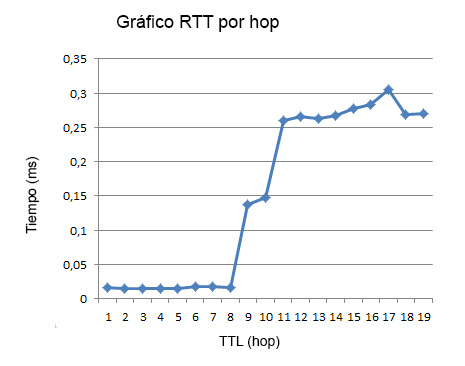
\includegraphics[width=0.7\textwidth]{img_analisis3/grafico-rtt-promedio.jpg} 
    \caption{Figura 1: $RTT$ promedio - Universidad de Hamburgo}	
	\end{center} 
\end{figure}

\begin{figure}[h]
	\begin{center}
    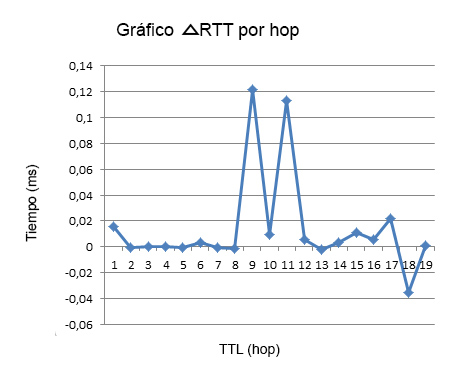
\includegraphics[width=0.7\textwidth]{img_analisis3/grafico-delta-rtt-promedio.jpg} 
    \caption{Figura 1: $\Delta RTT$ promedio - Universidad de Hamburgo}	
	\end{center} 
\end{figure}
%\newline
\newpage

De la muestra obtuvimos que los $\Delta RTT$ sigen una distribuci\'on Normal y que los enlaces submarinos, según los outliers obtenidos mediante el test de Grubbs, se corresponden con el salto 9 y el 11.
\\
Al observar los gráficos podemos notar que los resultados obtenidos mediante el test de Grubbs son correctos, ya que del salto 8 al 9 el paquete enviado viaja, según la geolocalización de las IP, desde Buenos Aires a Miami y su RTT promedio aumenta significativamente, y del salto 10 al 11 el paquete viaja de Miami a Frankfurt donde también hay un cambio abruto de su RTT promedio.
\\
Finalmente presentamos un mapa global donde vamos a trazar los puntos importantes de la ruta que realizan los paquetes. 
\newpage
\begin{figure}[h]
	\begin{center}
    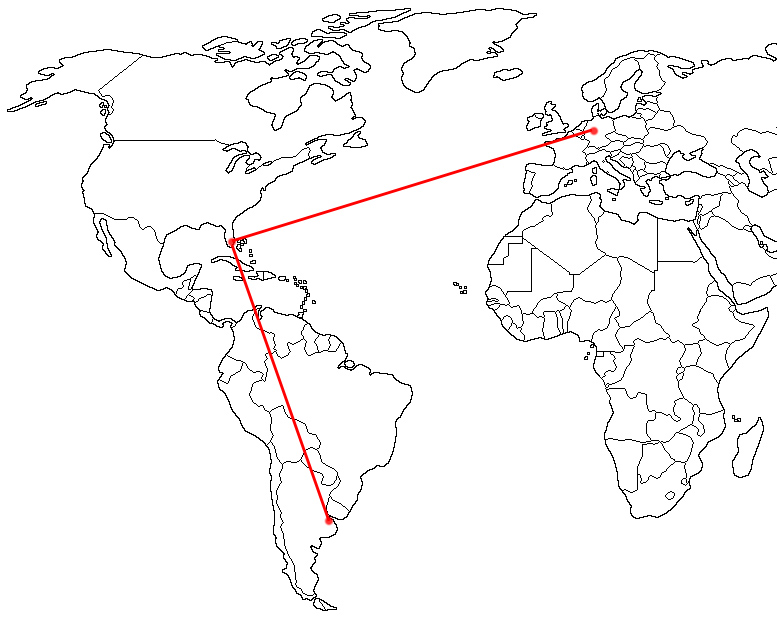
\includegraphics[width=0.7\textwidth]{img_analisis3/mapa.jpg} 
    \caption{Figura 1: Ruta del paquete - Universidad de Hamburgo}	
	\end{center} 
\end{figure}

